%%%%%% changing some paramaters in chunks
%%% name
%%% figure
%%% echo

\documentclass[11pt]{article}

\title{My first replicable Paper}
\author{
        MyFirstName MyLastName\\
        Evans School of Public Policy and Governance\\
        University of Washington\\
        Seattle, WA 98115, \underline{United States}\\
        \texttt{greatguy@uw.edu}
}
\date{\today}


\usepackage{Sweave}
\begin{document}
\Sconcordance{concordance:PaperInR_3.tex:PaperInR_3.Rnw:%
1 18 1 1 0 26 1 1 7 6 1 1 3 5 0 1 2 1 1 2 2 7 1 1 2 10 0 1 2 1 1 2 2 10 %
1 2 2 8 1 2 2 5 1}


\maketitle 

\begin{abstract}
This is an example on how to make a reproducible paper. We are using R from Rstudio, creating an RSweave document. This is a nice start to create a nice paper and get an A+. The next sections will show the steps taken.
\end{abstract}


\section{Introduction}\label{intro}

This is my intro to my great paper, I will explain the cool things I can do with my new `computational thinking' powers combined with some Latex. This is my intro to my great paper, I will explain the cool things I can do with my new `computational thinking' powers combined with some Latex. This is my intro to my great paper, I will explain the cool things I can do with my new `computational thinking' powers combined with some Latex. This is my intro to my great paper, I will explain the cool things I can do with my new `computational thinking' powers combined with some Latex.

This is my nice intro to my great paper, 
I will explain the cool things 
I can do with my new `computational thinking' 
powers
combined with some Latex.


\section{Exploring Data}\label{explo}


Sections may use a label\footnote{In fact, you can have a label wherever you think a future reference to that content might be needed.}. This label is needed for referencing. For example the next section has label \emph{datas}, so you can reference it by writing: As we see in section \ref{catexplo}.

% code chunk changes

\subsection{Exploring Categorical Data}\label{catexplo}

Here, I continue doing this nice work, I hope you like it and read it. It has been a very hard work.Here, I continue doing this nice work, I hope you like it and read it. It has been a very hard work.Here, I continue doing this nice work, I hope you like it and read it. It has been a very hard work.Here, I continue doing this nice work, I hope you like it and read it. It has been a very hard work.Here, I continue doing this nice work, I hope you like it and read it. It has been a very hard work.Here, I continue doing this nice work, I hope you like it and read it. It has been a very hard work.Here, I continue doing this nice work, I hope you like it and read it. It has been a very hard work.Here, I continue doing this nice work, I hope you like it and read it. It has been a very hard work.Here, I continue doing this nice work, I hope you like it and read it. It has been a very hard work.

% code chunk changes

\begin{Schunk}
\begin{Soutput}
 nd  ne per sel sub 
  2  41   8  21   4 
\end{Soutput}
\end{Schunk}

% code chunk changes
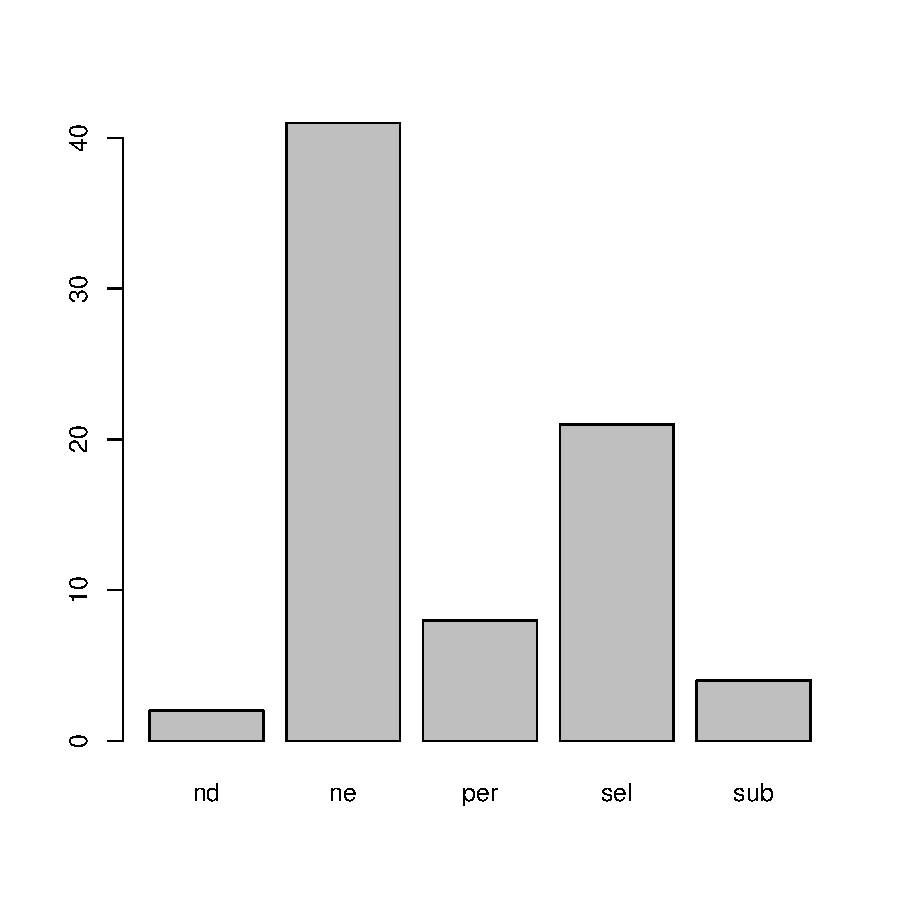
\includegraphics{PaperInR_3-cat_barplot}



\subsection{Exploring Numerical Data}\label{numexplo}

Here, I continue doing this nice work, I hope you like it and read it. It has been a very hard work.Here, I continue doing this nice work, I hope you like it and read it. It has been a very hard work.Here, I continue doing this nice work, I hope you like it and read it. It has been a very hard work.Here, I continue doing this nice work, I hope you like it and read it. It has been a very hard work.Here, I continue doing this nice work, I hope you like it and read it. It has been a very hard work.Here, I continue doing this nice work, I hope you like it and read it. It has been a very hard work.Here, I continue doing this nice work, I hope you like it and read it. It has been a very hard work.Here, I continue doing this nice work, I hope you like it and read it. It has been a very hard work.Here, I continue doing this nice work, I hope you like it and read it. It has been a very hard work.

% code chunk changes
\begin{Schunk}
\begin{Soutput}
       FH             RWB       
 Min.   :10.00   Min.   : 6.38  
 1st Qu.:43.50   1st Qu.:28.22  
 Median :61.00   Median :37.99  
 Mean   :58.91   Mean   :39.67  
 3rd Qu.:80.00   3rd Qu.:46.85  
 Max.   :97.00   Max.   :83.90  
\end{Soutput}
\end{Schunk}

% code chunk changes
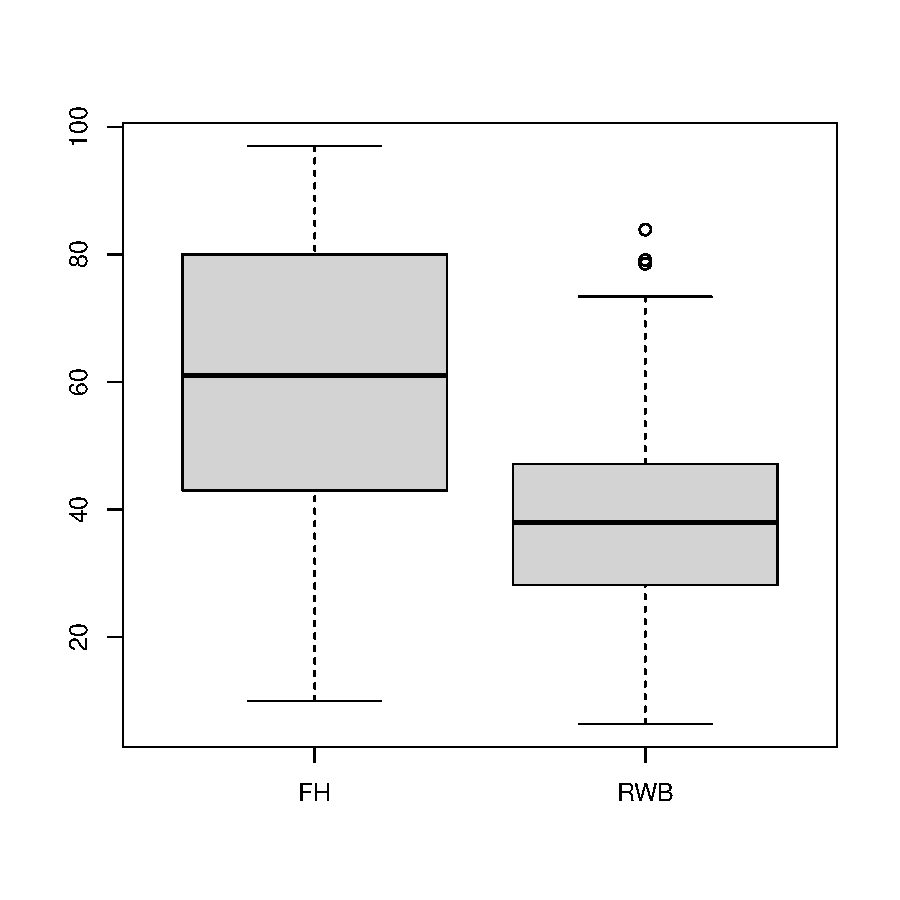
\includegraphics{PaperInR_3-num_plot}

Boxplots were introduced by Tuckey (Tukey, John W (1977). Exploratory Data Analysis. Addison-Wesley.)

\section{Looking for Relationships}\label{bivar}


Here, I continue doing this nice work, I hope you like it and read it. It has been a very hard work.Here, I continue doing this nice work, I hope you like it and read it. It has been a very hard work.Here, I continue doing this nice work, I hope you like it and read it. It has been a very hard work.Here, I continue doing this nice work, I hope you like it and read it. It has been a very hard work.Here, I continue doing this nice work, I hope you like it and read it. It has been a very hard work.Here, I continue doing this nice work, I hope you like it and read it. It has been a very hard work.Here, I continue doing this nice work, I hope you like it and read it. It has been a very hard work.Here, I continue doing this nice work, I hope you like it and read it. It has been a very hard work.Here, I continue doing this nice work, I hope you like it and read it. It has been a very hard work.

\subsection{Numerical and  Categorical}\label{binumcat}

% code chunk changes
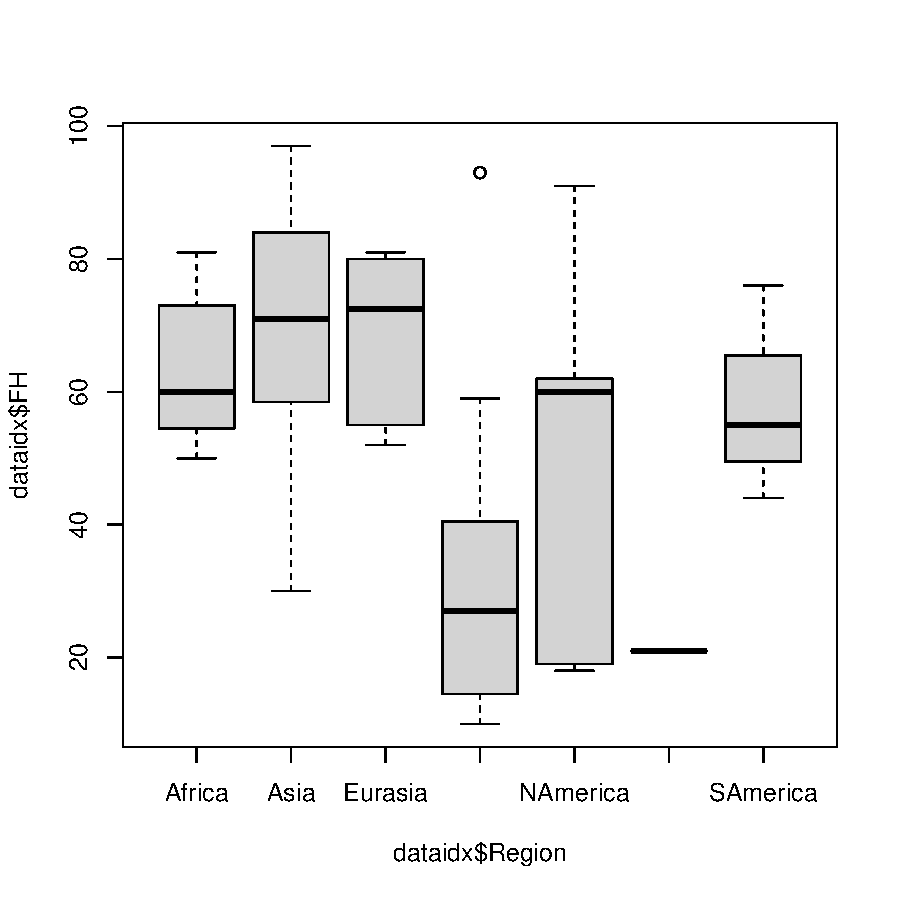
\includegraphics{PaperInR_3-numcat_plot}

Here, I continue doing this nice work, I hope you like it and read it. It has been a very hard work.Here, I continue doing this nice work, I hope you like it and read it. It has been a very hard work.Here, I continue doing this nice work, I hope you like it and read it. It has been a very hard work.Here, I continue doing this nice work, I hope you like it and read it. It has been a very hard work.Here, I continue doing this nice work, I hope you like it and read it. It has been a very hard work.Here, I continue doing this nice work, I hope you like it and read it. It has been a very hard work.Here, I continue doing this nice work, I hope you like it and read it. It has been a very hard work.Here, I continue doing this nice work, I hope you like it and read it. It has been a very hard work.Here, I continue doing this nice work, I hope you like it and read it. It has been a very hard work.

\subsection{Numerical and Numerical}\label{binumnum}

Here, I continue doing this nice work, I hope you like it and read it. It has been a very hard work.Here, I continue doing this nice work, I hope you like it and read it. It has been a very hard work.Here, I continue doing this nice work, I hope you like it and read it. It has been a very hard work.Here, I continue doing this nice work, I hope you like it and read it. It has been a very hard work.Here, I continue doing this nice work, I hope you like it and read it. It has been a very hard work.Here, I continue doing this nice work, I hope you like it and read it. It has been a very hard work.Here, I continue doing this nice work, I hope you like it and read it. It has been a very hard work.Here, I continue doing this nice work, I hope you like it and read it. It has been a very hard work.Here, I continue doing this nice work, I hope you like it and read it. It has been a very hard work.
%%%%%% code for exploring here

% code chunk changes
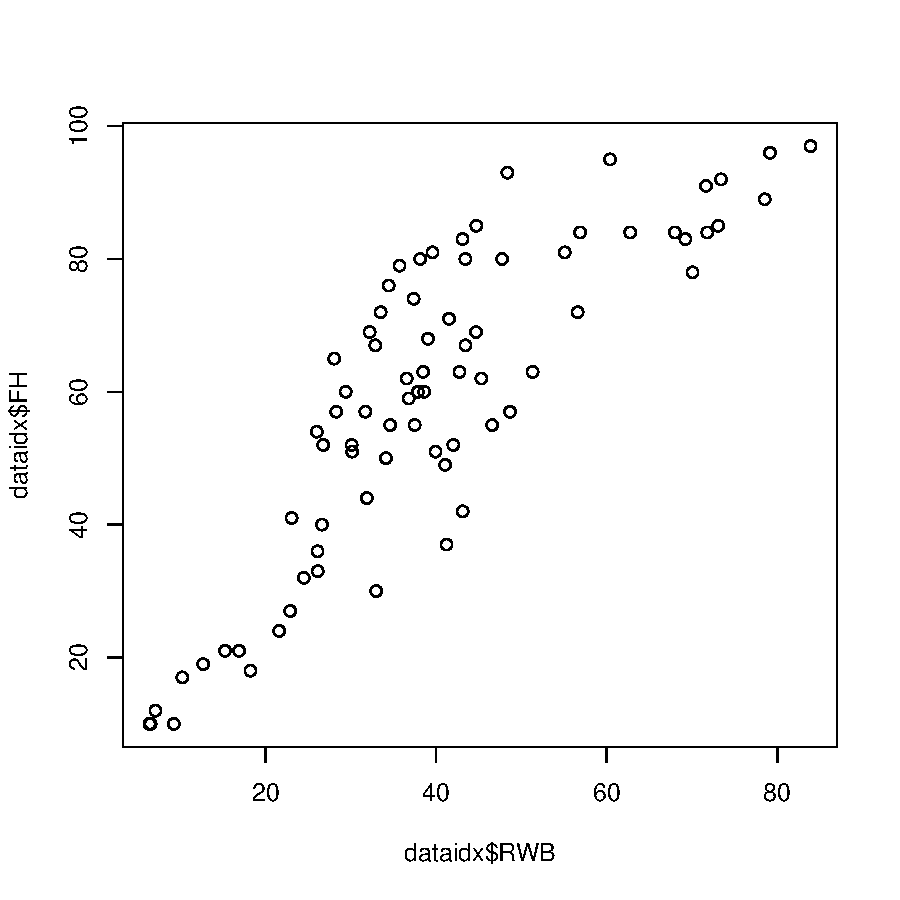
\includegraphics{PaperInR_3-numnum_plot}

The scatter plot is thought to be invented by  John Frederick W. Herschel according to this link: https://qz.com/1235712/the-origins-of-the-scatter-plot-data-visualizations-greatest-invention/



\end{document}
